
\section{Architecture Integration}

\subsection{Model Support}

\begin{table}[H]
\centering
\small
\begin{tabular}{lllll}
\toprule
\textbf{Architecture} & \textbf{Projections} & \textbf{Attention} & \textbf{Conv1D?} & \textbf{Nested?} \\
\midrule
DistilBERT-base & \texttt{q\_lin, k\_lin, v\_lin, out\_lin} & Flat MHA & No & No \\
RoBERTa-base & \texttt{query, key, value, output.dense} & Nested & No & Yes \\
GPT-2 & \texttt{c\_attn} (fused), \texttt{c\_proj} & Causal Conv1D & Yes & No \\
Qwen3.5-0.8B & \texttt{q\_proj, k\_proj, v\_proj, o\_proj} & GQA + RoPE & No & No \\
\bottomrule
\end{tabular}
\end{table}

\subsection{Weight Transfer}

\subsubsection{DistilBERT (Flat)}

Direct copy from \texttt{q\_lin}, \texttt{k\_lin}, \texttt{v\_lin}, \texttt{out\_lin}. Each weight is 
factorized via CUR.

\begin{lstlisting}
target.q\_proj.copy\_cur(src.q\_lin.weight, src.q\_lin.bias)
target.k\_proj.copy\_cur(src.k\_lin.weight, src.k\_lin.bias)
target.v\_proj.copy\_cur(src.v\_lin.weight, src.v\_lin.bias)
target.out\_proj.copy\_cur(src.out\_lin.weight, src.out\_lin.bias)
\end{lstlisting}

\subsubsection{RoBERTa (Nested)}

Extract from \texttt{self.query}, \texttt{self.key}, \texttt{self.value}, \texttt{output.dense}.

\begin{lstlisting}
target.q\_proj.copy\_cur(src.self.query.weight, src.self.query.bias)
target.k\_proj.copy\_cur(src.self.key.weight, src.self.key.bias)
target.v\_proj.copy\_cur(src.self.value.weight, src.self.value.bias)
# out\_proj is bypassed via is\_nested\_encoder = True
\end{lstlisting}

\subsubsection{GPT-2 (Conv1D)}

GPT-2 fuses Q, K, V into \texttt{c\_attn}:

\begin{lstlisting}
w = src.c\_attn.weight.t()  # Conv1D stores (in, out) $\to$ transpose
q\_w, k\_w, v\_w = w.chunk(3, dim=0)
target.q\_proj.copy\_cur(q\_w, q\_bias)
target.k\_proj.copy\_cur(k\_w, k\_bias)
target.v\_proj.copy\_cur(v\_w, v\_bias)
target.out\_proj.copy\_cur(src.c\_proj.weight.t(), src.c\_proj.bias)
\end{lstlisting}

\subsubsection{Qwen3.5 (GQA)}

Direct copy with GQA-preserving shapes.

\subsection{Handling Nested Encoders}

RoBERTa's attention sits inside \texttt{BertAttention}:

\begin{lstlisting}
class BertAttention:
    self: BertSelfAttention      # query, key, value
    output: BertSelfOutput       # dense (output projection)
\end{lstlisting}

PHANTOM replaces \texttt{attention.self} and sets \texttt{is\_nested\_encoder = True}. The 
forward pass returns raw context without applying \texttt{out\_proj}, letting the 
outer \texttt{BertSelfOutput.dense} handle the projection.

\subsection{Handling GQA}

For GQA models ($H_{kv} < H$):

\begin{lstlisting}
if self.num\_heads != self.num\_kv\_heads:
    repeats = self.num\_heads // self.num\_kv\_heads
    K = repeat\_kv(K, repeats)
    V = repeat\_kv(V, repeats)
\end{lstlisting}

Applied after projection, before attention.

\subsection{Handling RoPE}

For models with RoPE (Qwen, LLaMA):

\begin{lstlisting}
if position\_embeddings is not None:
    cos, sin = position\_embeddings
    Q, K = apply\_rotary\_pos\_emb(Q, K, cos, sin)
\end{lstlisting}

Applied after projection, before GQA expansion.

\subsection{Injection Algorithm}

\textbf{Algorithm 2:} Inject PHANTOM into a model
\begin{lstlisting}
Input:  model M, config c
Output: M' with attention replaced

1:  for layer   in transformer\_layers(M):
2:      src $\leftarrow$ extract\_attention( )
3:      if src is None: continue
4:      new $\leftarrow$ PHANTOMAttention(c, old=src)
5:      new.copy\_weights(src)
6:      replace\_attention( , new)
7:  end for
8:  return M'
\end{lstlisting}

\subsection{The `FactorisedLinear\_CUR` Module}

\begin{lstlisting}
class FactorisedLinear\_CUR(nn.Module):
    def \_\_init\_\_(self, in\_features, out\_features, cur\_rank=16, ...):
        super().\_\_init\_\_()
        self.down = nn.Linear(in\_features, cur\_rank, bias=False)
        self.up = nn.Linear(cur\_rank, out\_features, bias=bias)
        # Optional LoRA
        if lora\_rank \textgreater{} 0:
            self.lora\_A = nn.Parameter(torch.empty(lora\_rank, in\_features))
            self.lora\_B = nn.Parameter(torch.zeros(out\_features, lora\_rank))
    
    def copy\_cur(self, weight, bias):
        # 1. SVD
        U, S, Vt = torch.linalg.svd(weight)
        # 2. Leverage scores
        col\_lev = (Vt ** 2).sum(dim=0)
        row\_lev = (U ** 2).sum(dim=1)
        # 3. Top-r selection
        col\_idx = torch.topk(col\_lev, k=rank).indices
        row\_idx = torch.topk(row\_lev, k=rank).indices
        # 4. CUR factors
        C = weight[:, col\_idx]
        R = weight[row\_idx, :]
        W\_int = weight[row\_idx][:, col\_idx]
        # 5. Assign
        self.down.weight.data = R
        self.up.weight.data = C @ torch.linalg.pinv(W\_int)
    
    def forward(self, x):
        out = self.up(self.down(x))
        if self.lora\_rank \textgreater{} 0:
            out += F.linear(F.linear(x, self.lora\_A), self.lora\_B) * self.lora\_scaling
        return out * self.output\_scale
\end{lstlisting}

\subsection{LSH Attention Module}

\begin{lstlisting}
def lsh\_attention(Q, K, V, rounds=4, bucket\_size=4, softpick\_temp=1.0, ...):
    B, H, N, D = Q.shape
    scale = D ** -0.5
    n\_bits = min(bucket\_size, 8)
    bit\_shifts = torch.tensor([2**i for i in range(n\_bits)])
    
    Q\_norm = F.normalize(Q, p=2, dim=-1)
    K\_norm = F.normalize(K, p=2, dim=-1)
    
    scores = torch.matmul(Q.float(), K.float().transpose(-2, -1)) * scale
    # ... masking ...
    
    accum = torch.zeros\_like(V)
    for \_ in range(rounds):
        proj = F.normalize(torch.randn(D, n\_bits), p=2, dim=0)
        hq = (Q\_norm @ proj \textgreater{} 0).float() @ bit\_shifts
        hk = (K\_norm @ proj \textgreater{} 0).float() @ bit\_shifts
        match = (hq.unsqueeze(-1) == hk.unsqueeze(-2)) | eye
        scores\_r = scores.masked\_fill(~match, -1e4)
        alpha = softpick(scores\_r, dim=-1, temperature=softpick\_temp)
        accum += alpha @ V
    
    return accum / rounds
\end{lstlisting}

\subsection{Fallback and Error Handling}

\begin{table}[H]
\centering
\small
\begin{tabular}{lll}
\toprule
\textbf{Failure} & \textbf{Detection} & \textbf{Response} \\
\midrule
SVD failure & Exception & Kaiming init \\
Pseudoinverse failure & NaN/Inf & Kaiming init \\
Missing weights & \texttt{copy\_weights} raises & Skip layer \\
Shape mismatch & Assertion & Skip layer \\
Frobenius norm \textless{} 1e-4 & Check after copy & Raise error \\
\bottomrule
\end{tabular}
\end{table}

\subsection{Registry}

\begin{lstlisting}
@ATTENTION\_REGISTRY.register("phantom")
@ATTENTION\_REGISTRY.register("phantom\_module")
class PHANTOMAttention(BaseAttention):
    ...
\end{lstlisting}

\subsection{Causality Verification}

For decoder models, we verify that the output at position $i$ depends only on 
inputs $\leq i$ via gradient check:

\begin{lstlisting}
X = torch.randn(1, N, d, requires\_grad=True)
Y = model(X)
Y[0, i].sum().backward()
assert X.grad[0, i+1:].abs().max() \textless{} 1e-6
\end{lstlisting}
\begin{lstlisting}

---
\end{lstlisting}

\begin{figure}[H]
\centering
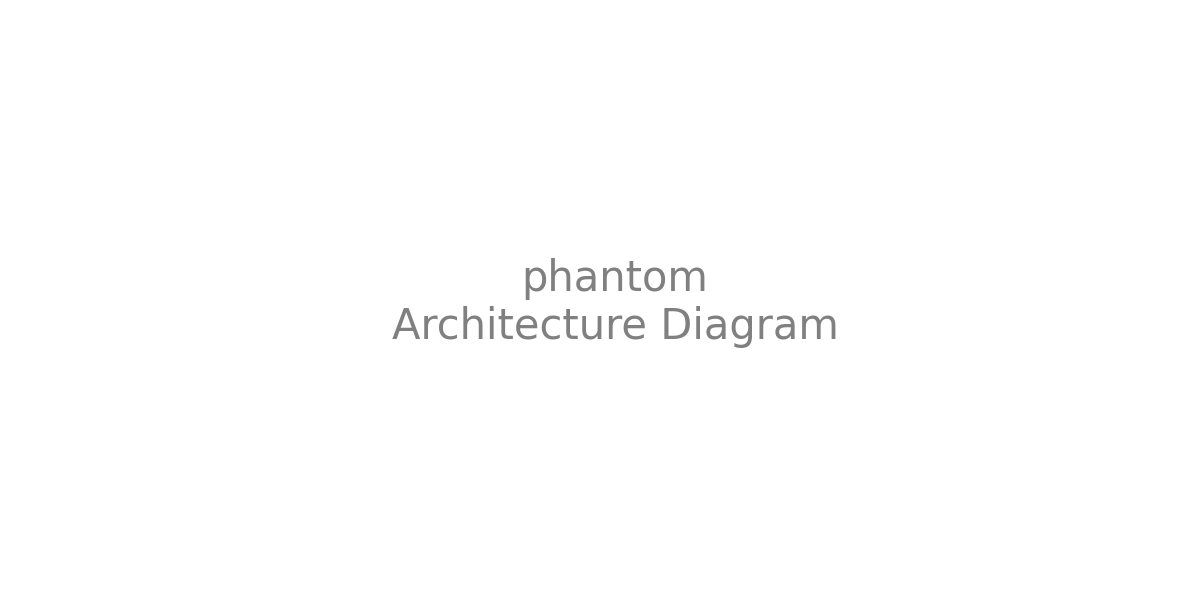
\includegraphics[width=\linewidth]{figures/architecture.png}
\caption{High-level architectural diagram of phantom.}
\label{fig:arch_phantom}
\end{figure}

